\documentclass[t]{beamer}

\usetheme{TuringLight}
%\usetheme{TuringDark}

% Presentation data
\subtitle{Enrichment experience}
\date{31/03/2023}
\author{Susana Roman Garcia, PhD student, University of Edinburgh.}

% Uncomment any of these lines below to set custom size for each of the font sizes.
% The default value is shown in the comment.
%\setlength{\titlefontsize}{6.875\basefontsize}
%\setlength{\subtitlefontsize}{4.375\basefontsize}
%\setlength{\frametitlesize}{2.625\basefontsize}
%\setlength{\framesubtitlesize}{1.625\basefontsize}
%\setlength{\bodytextsize}{2\basefontsize}
%\setlength{\blocktitlesize}{\bodytextsize}
%\setlength{\blockbodysize}{\bodytextsize}

% Start document
\begin{document}

% Title slide (details filled from presentation data fields above)
\begin{frame}
	\titlepage
\end{frame}

% Imprint slide (e.g. about the institute / opening quote)
\begin{frame}{9 months placement (Oct 2022 - Jun 2023) So not done yet!}
    \begin{itemize}
        \item What have I been up to? Were my goals achieved? 
        \item What have I actually done?
        \item What have I gained from this experience so far?
    \end{itemize}
\end{frame}

\begin{frame}{Contents}
	\tableofcontents
\end{frame}

% Section divider slide
\section{1.Original ideas}
\subsection{1.1. What did I have in mind before joining the scheme?}
\begin{frame}{1.1. What did I have in mind before joining the scheme?}
    \begin{block}{"Explore reproducibility and bias by designing seminars and workshops with people knowledgeable in different fields. E.g., workshop where people with expertise in research of Ethics and people researching in Computational Neuroscience come together."}
    \end{block}    

\end{frame}

\section{2. Bringing ideas into action}
\subsection{2.1. How do I collaborate with people here?}
\begin{frame}{2.1. How do I collaborate with people here?}
	\begin{block}{I wanted to: Collaborate with others to talk about ethics and bias in research}
  		\begin{itemize}    
  			\item \textbf{October (and previously):} Lots of talks with Turing Way, Tools, Practices and Systems and Turing Commons people...
                \item \textbf{October:} Met Ceilidh Welsh <3
  			\item \textbf{November:} Pitched the idea of doing a workshop (which transformed into a one-day symposium).
                \item \textbf{December:} Planning started. Lots of Zoom calls.
  		\end{itemize}    
	\end{block}
 
\end{frame}

\subsection{2.2. Planning the Data Hazards, Ethics and Reproducibility Symposium}
\begin{frame}{2.2. Planning the Data Hazards, Ethics and Reproducibility Symposium}
	\begin{block}{Using the grassroots funding: organising a one-day symposium at the Turing HQ.}
            \begin{columns}[T,totalwidth=\textwidth]
  		\begin{column}{0.45\textwidth}
                \begin{figure}
				\vspace{-\blocktitlesize}
\includegraphics[height=0.5\paperheight,keepaspectratio]{data_hazards.JPG}
			\end{figure}
            \end{column}
            
            \begin{column}{0.6\textwidth}
            \begin{itemize}  
                \item<2-> \textbf{November - December:} road maps, work-back plans, polls for interest, brain storming of tasks required like facilitators, volunteers, hybrid logistics.
  			\item<3-> \textbf{January - February:} agenda preparation, contacted speakers, spread the message that the event is happening, catering...
                \item<4-> \textbf{March: 10th March was the date!}
  		\end{itemize}  
            \end{column}%
            \end{columns}
	\end{block}
\end{frame}

\begin{frame}
    \begin{figure}
        \vspace{-\blocktitlesize}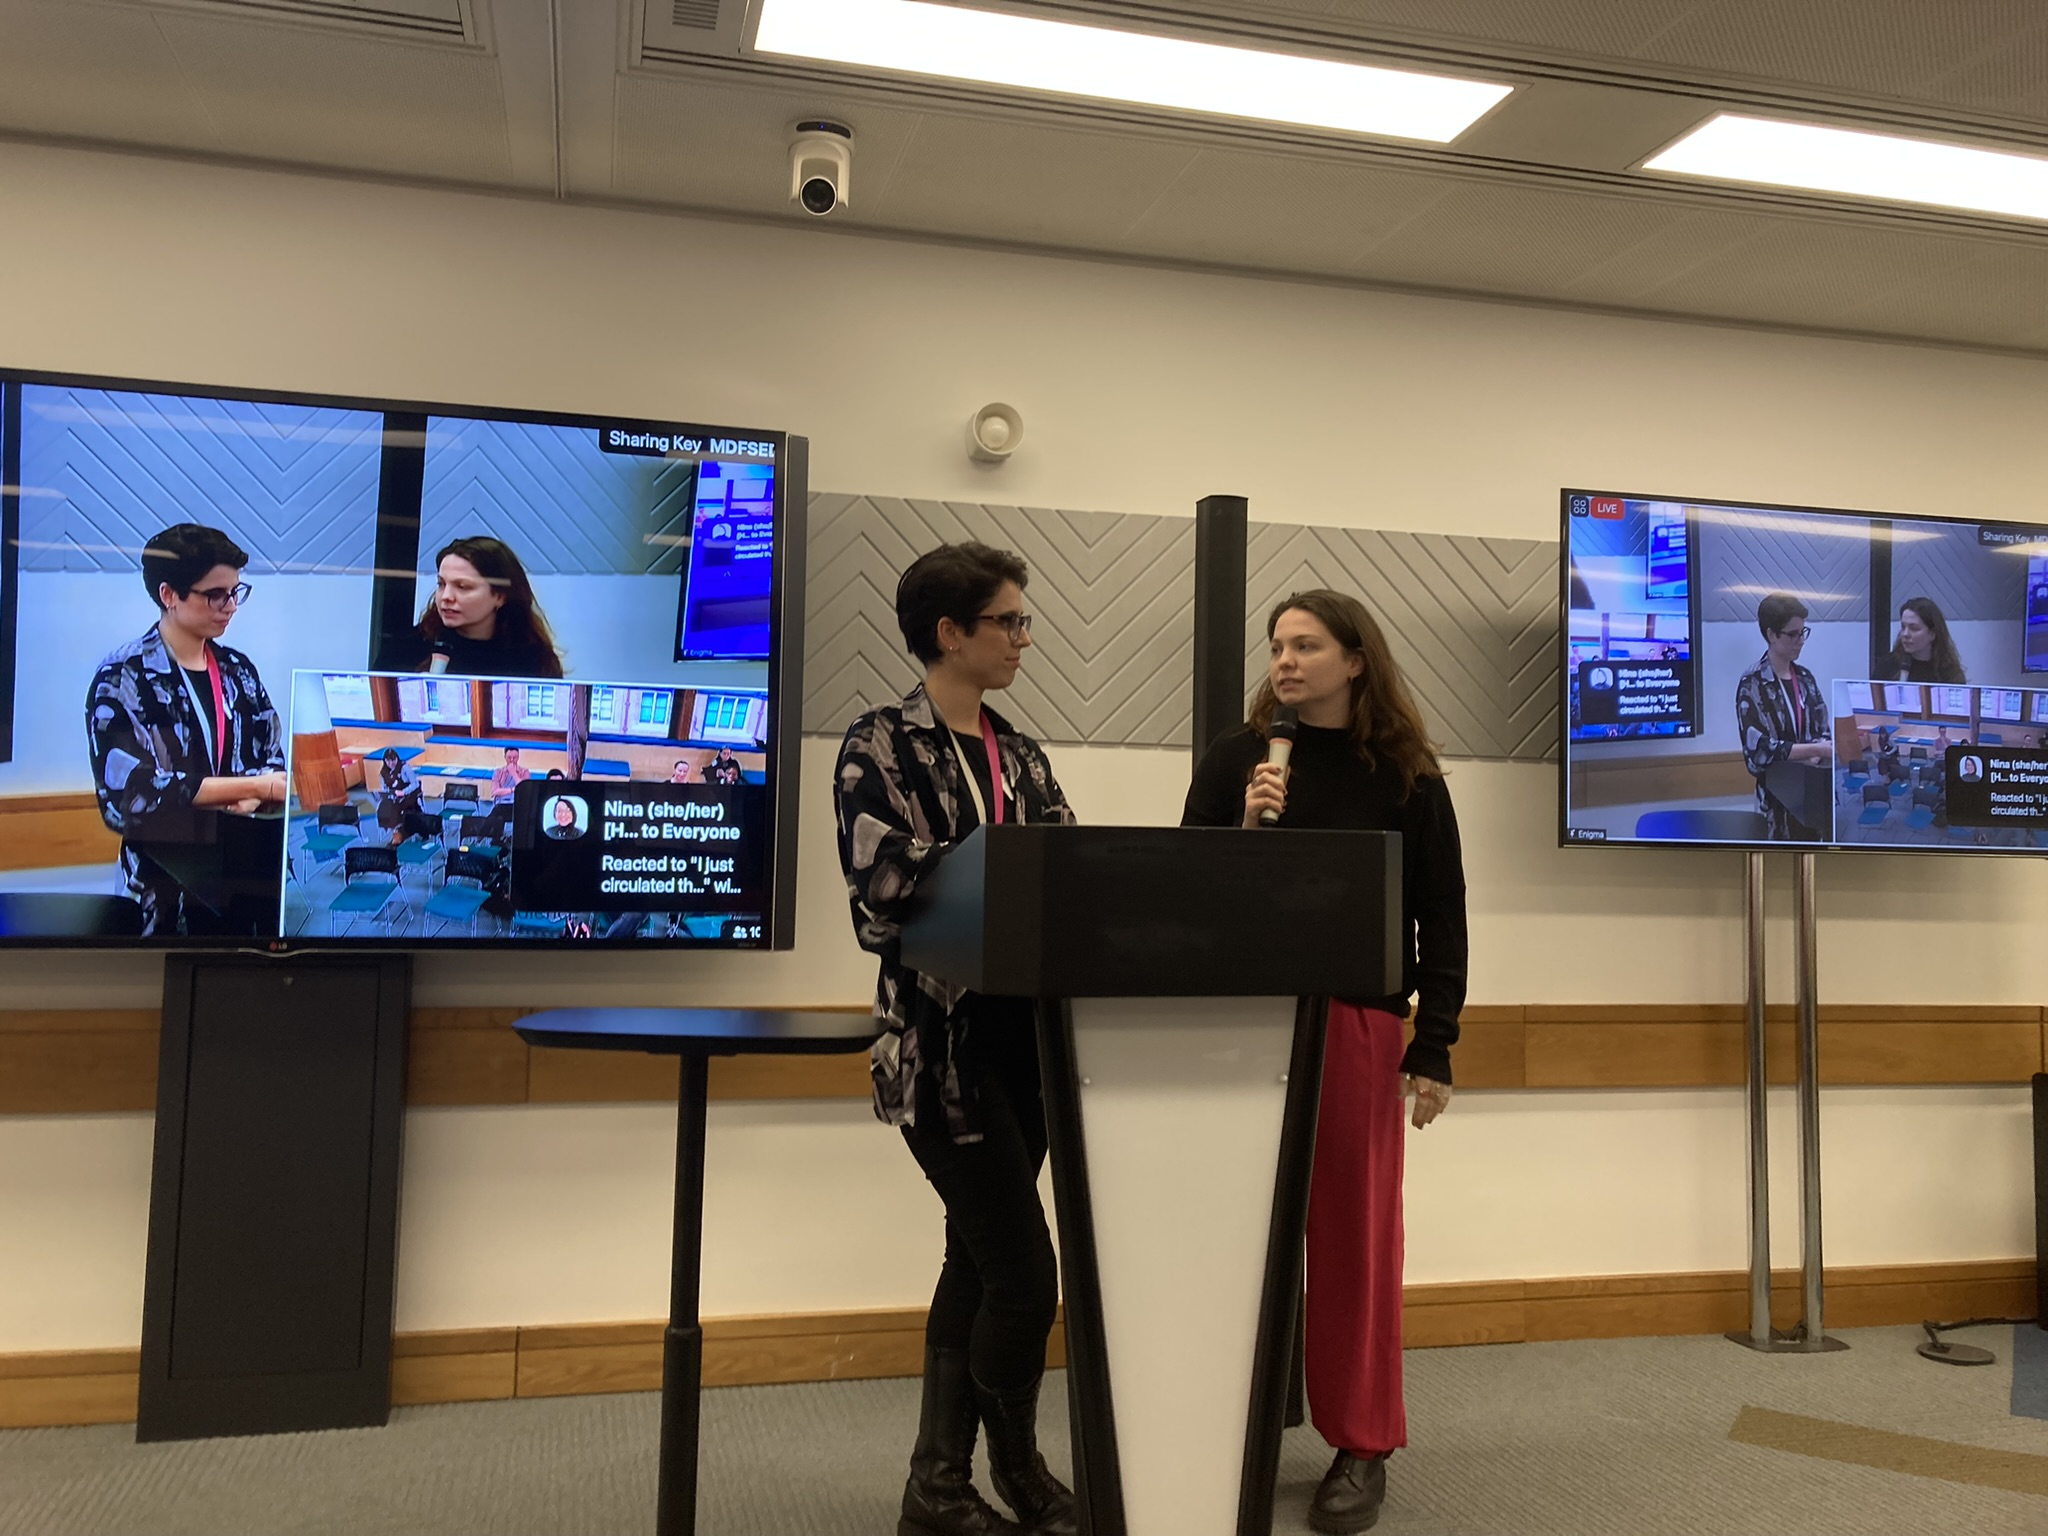
\includegraphics[height=0.8\paperheight,keepaspectratio]{susana_ceilidh.jpeg}
    \end{figure}
\end{frame}

\begin{frame}
    \begin{figure}
        \vspace{-\blocktitlesize}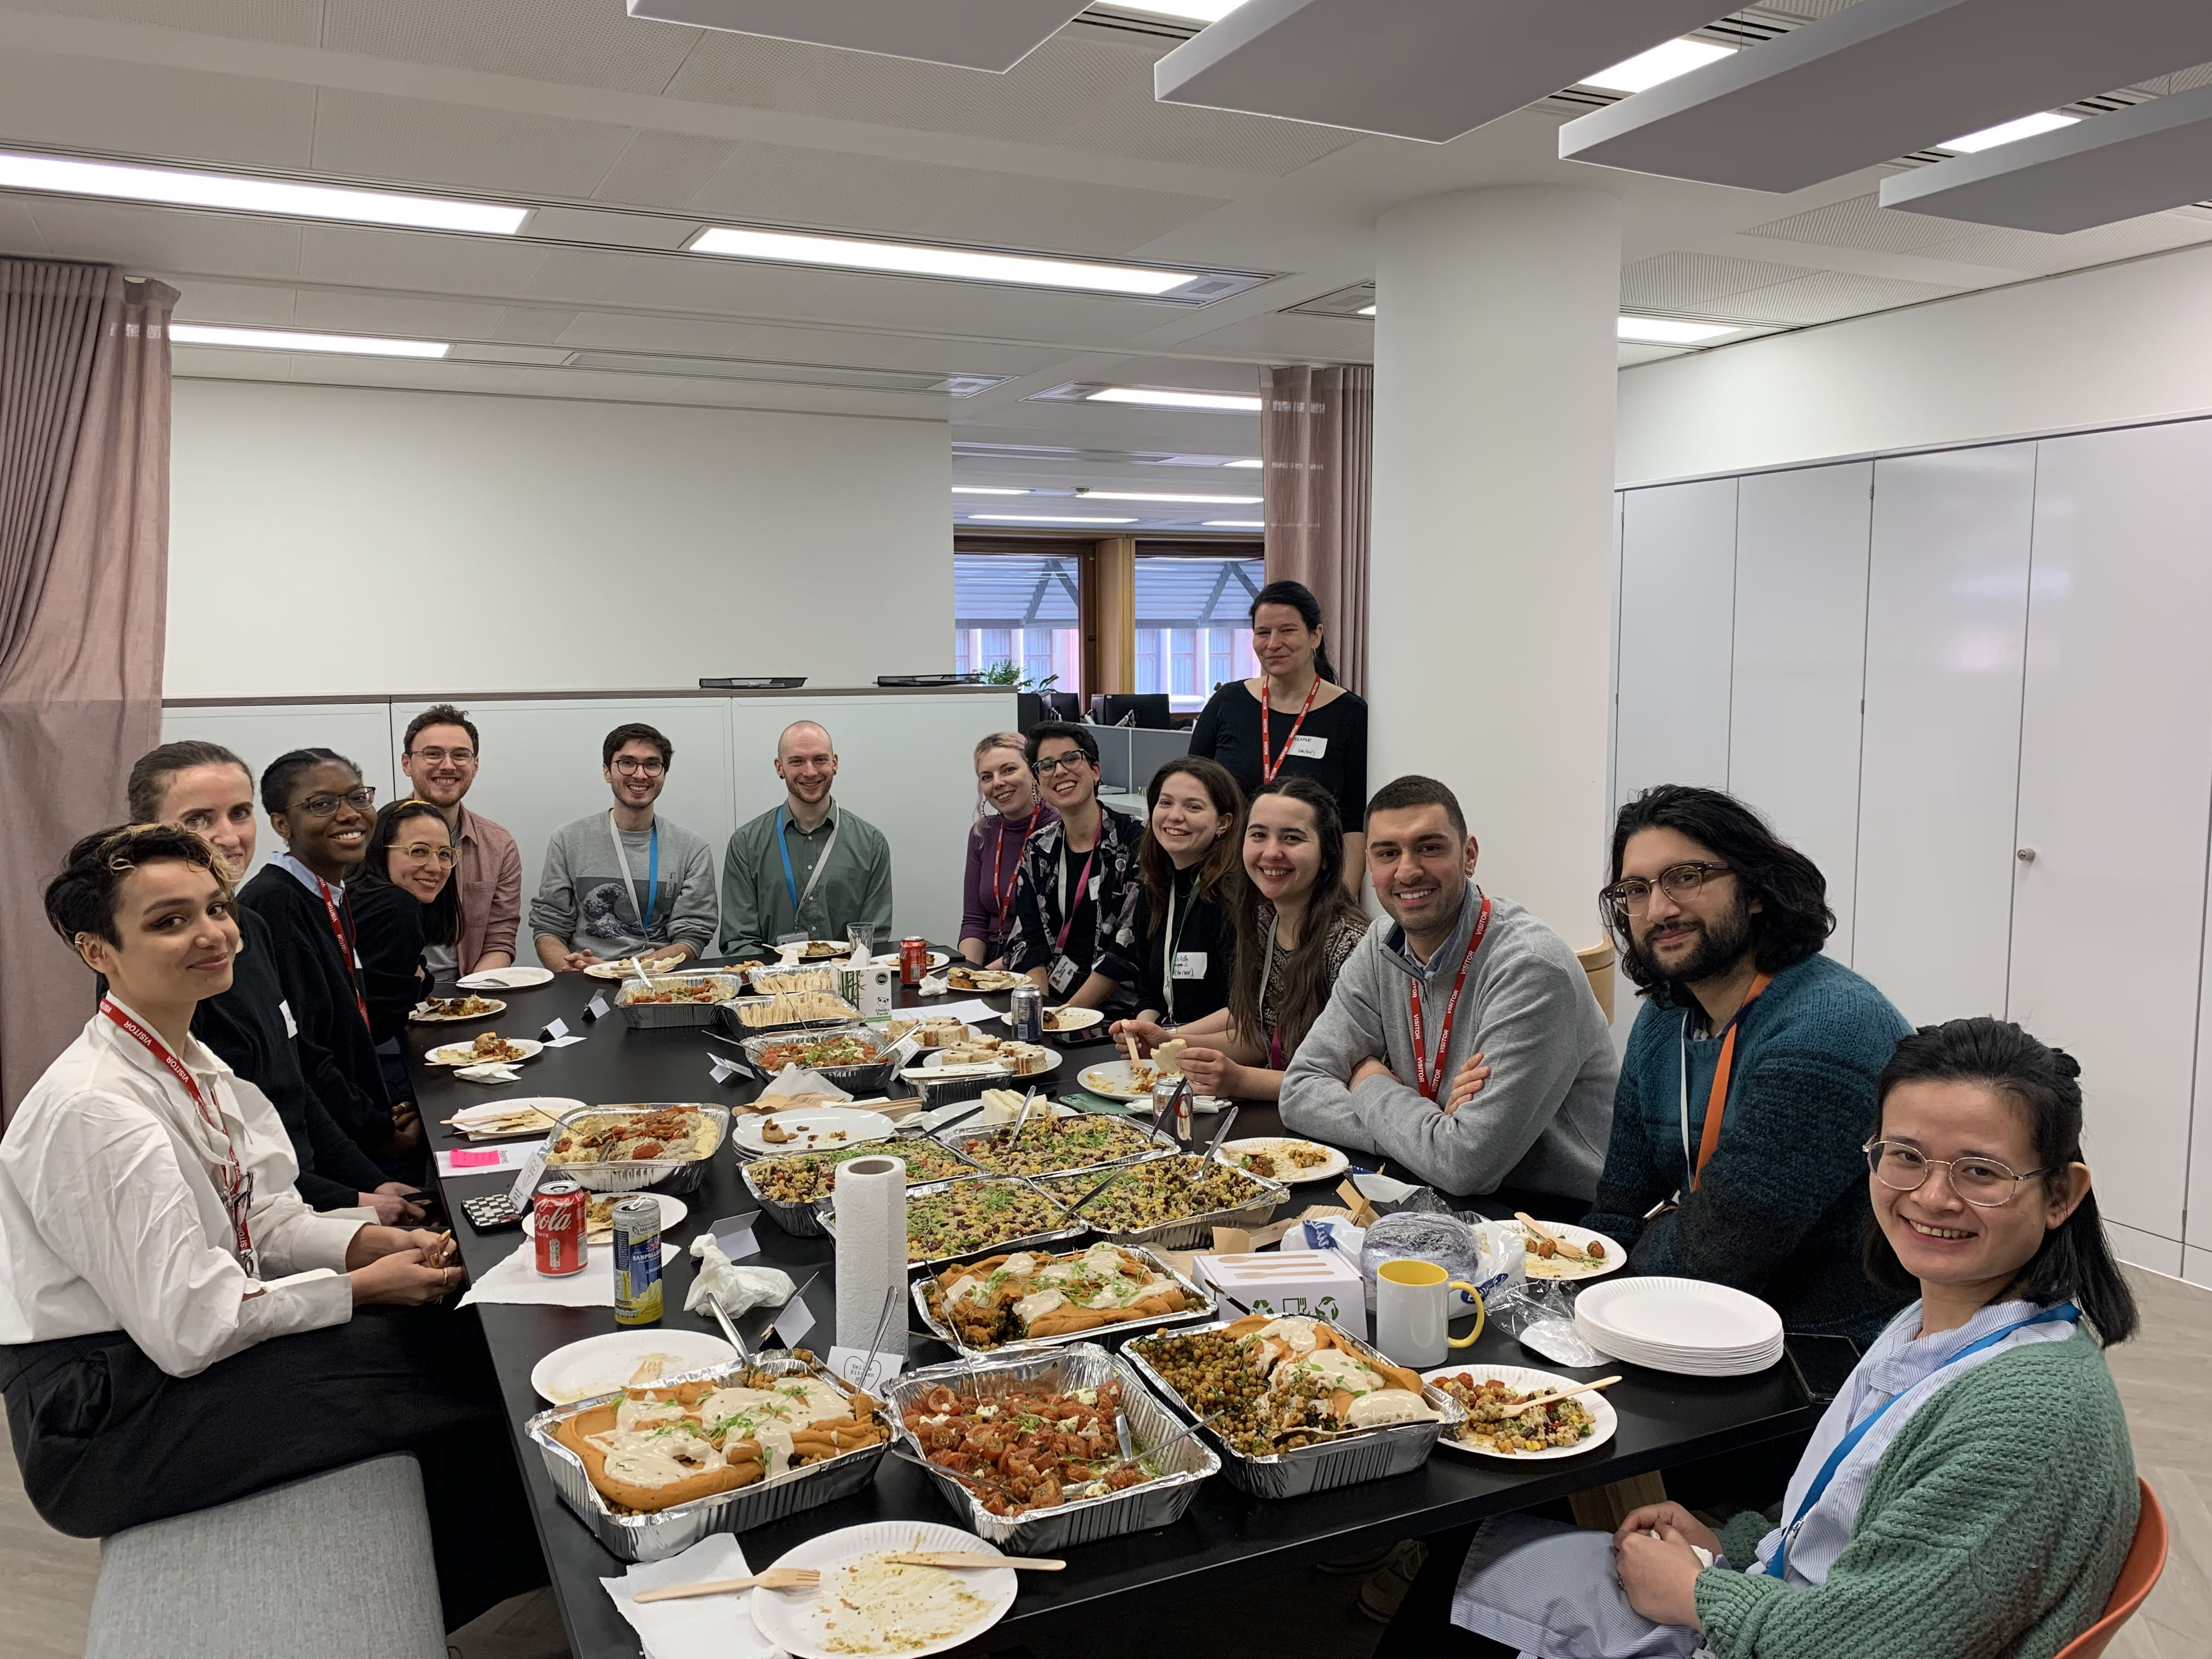
\includegraphics[height=0.8\paperheight,keepaspectratio]{der_20230310.jpg}
    \end{figure}
\end{frame}

\subsection{2.3. What else? A lot more!}
\begin{frame}{2.3. What else? A lot more!}
	\begin{block}{Research Software Engineering with Python (2 weeks in October)}
  		\begin{itemize}    
  			\item Tried to learn how to construct more reliable, readable, efficient research software in a collaborative environment.
  		\end{itemize}    
	\end{block}
 
        \begin{block}{Open Life Sciences Cohort (16 weeks training, October - January)}
  		\begin{itemize}    
  			\item Topics on openness, open science, open leadership, community interactions, value exchanges, inclusivity, accessibility, open Science practices in developing resources and training.
  		\end{itemize}    
	\end{block}

        \begin{block}{TTW Workshop in Newcastle, Collaboration Cafes, TPS chats, Community Events}
	\end{block}

 
\end{frame}

\section{3. Into the future}
\subsection{3.1. What projects am I doing next?}
% Skeleton double-column text slide (two text columns)
\begin{frame}{3.1. What projects am I doing next?}
  	\begin{block}{Had to drop: Project Collaboration the Turing Institute.}
    	\begin{itemize}    
    		\item Keyword extraction to create quantitative analysis of speciesist bias in Computational Neuroscience papers. 
    				\end{itemize}  
	\end{block}
 
  	\begin{block}{Re-work my actual PhD models with new acquired knowledge}
	\end{block}
        \begin{block}{Writing a chapter on Data Hazards in my PhD thesis}
	\end{block}
\end{frame}



% End slide 
\begin{frame}{Thank you for listening.}	
    \begin{itemize}
        \item Thank you, everyone, for all your hard work and kindness. 
        \item Thank you for the good times. 
        \item You are actually the best part of the experience at the Turing.
        \item Thank you for the friendships.
        \begin{figure}
				\vspace{-\blocktitlesize}
\includegraphics[height=0.5\paperheight,keepaspectratio]{qrcode.png}
			\end{figure}
    \end{itemize}
\end{frame}

\end{document}
